\begin{fact} \label{exp-cont}
    $\exp$ est continue sur $\RR$.
\end{fact}


\begin{proof}
    Fixons $x_0 \in \RR$, et considérons $\epsilon \in \intervalO{0}{\exp(x_0)}$ quelconque.
    Nous devons trouver $\eta \in \RRsp$ tel que
    $x_0 - \eta < x < x_0 + \eta$
    implique
    $\exp(x_0) - \epsilon < \exp x < \exp(x_0) + \epsilon$. Voici comment faire.
    %
    \begin{itemize}
        \item Par stricte croissance de $\ln$ et $\exp$, nous avons l'équivalence logique ci-dessous qui permet de comprendre ce qui va suivre.

        \noindent$
            0 < \exp(x_0) - \epsilon < \exp x < \exp(x_0) + \epsilon
            \iff
            \ln \big( \exp(x_0) - \epsilon \big) < x < \ln \big( \exp(x_0) + \epsilon \big)
        $


        \item
        $\ln \big( \intervalO{\exp(x_0) - \epsilon}{\exp(x_0) + \epsilon} \big)
        =
         \intervalO{\ln \big( \exp(x_0) - \epsilon \big)}{\ln \big( \exp(x_0) + \epsilon \big)}$,
         car $\ln$ est croissante sur $\RRsp$, et sa continuité permet de faire appel au \tvi, voir le \reffact{tvi}.
        %
        Nous noterons $I_{\epsilon}$ cet intervalle non vide.


        \item De $x_0 = \ln(\exp x_0)$, nous déduisons que $x_0 \in I_{\epsilon}$,
        puis le point précédent donne $\eta \in \RRsp$ tel que
        $\intervalO{x_0 - \eta}{x_0 + \eta} \subseteq I_{\epsilon}$.


        \item Les implications logiques suivantes permettent de conclure.

        \smallskip
        \leavevmode\kern-19pt\begin{stepcalc}[style=ar*, ope=\implies]
            x_0 - \eta < x < x_0 + \eta
        \explnext*{$\intervalO{x_0 - \eta}{x_0 + \eta} \subseteq I_{\epsilon}$}{}
            x \in I_{\epsilon}
        \explnext{}
            \ln \big( \exp(x_0) - \epsilon \big) < x < \ln \big( \exp(x_0) + \epsilon \big)
        \explnext{}
            \ln \big( \exp(x_0) - \epsilon \big) < \ln \big( \exp(x) \big) < \ln \big( \exp(x_0) + \epsilon \big)
        \explnext*{Stricte croissante de $\ln$.}{}
            \exp(x_0) - \epsilon < \exp x < \exp(x_0) + \epsilon
        \end{stepcalc}
    \end{itemize}

    \null
    \vspace{-4.5ex}
\end{proof}


% ----------------------- %


\begin{fact}
    $\forall x \in \RR$,
    $\sder{\exp}{1} x = \exp x$
    (ceci redonne la stricte croissance de $\exp$).%
    \footnote{
        Bien noter que nous n'avons pas utilisé la stricte croissance de $\exp$ dans la preuve du fait \ref{exp-cont} qui va servir à calculer $\sder{\exp}{1}$.
    }
\end{fact}


\begin{proof}
    Notons $\setproba{L}$ et $\setproba{E}$ les représentations graphiques respectives des fonctions $\ln$ et $\exp$.
    %
    Nous savons que $\setproba{L}$ et $\setproba{E}$ sont symétriques par rapport à la droite $\Delta: y = x$.
    Pour $h \neq 0$, considérons
    $A(a ; \exp a) \in \setproba{E}$ et $M(a+h ; \exp(a+h)) \in \setproba{E}$.
    Par symétrie, nous avons
    $B(\exp a ; a) \in \setproba{L}$ et $N(\exp(a+h) ; a+h) \in \setproba{L}$.
    %
    Nous arrivons à la situation graphique suivante.

    \begin{center}
        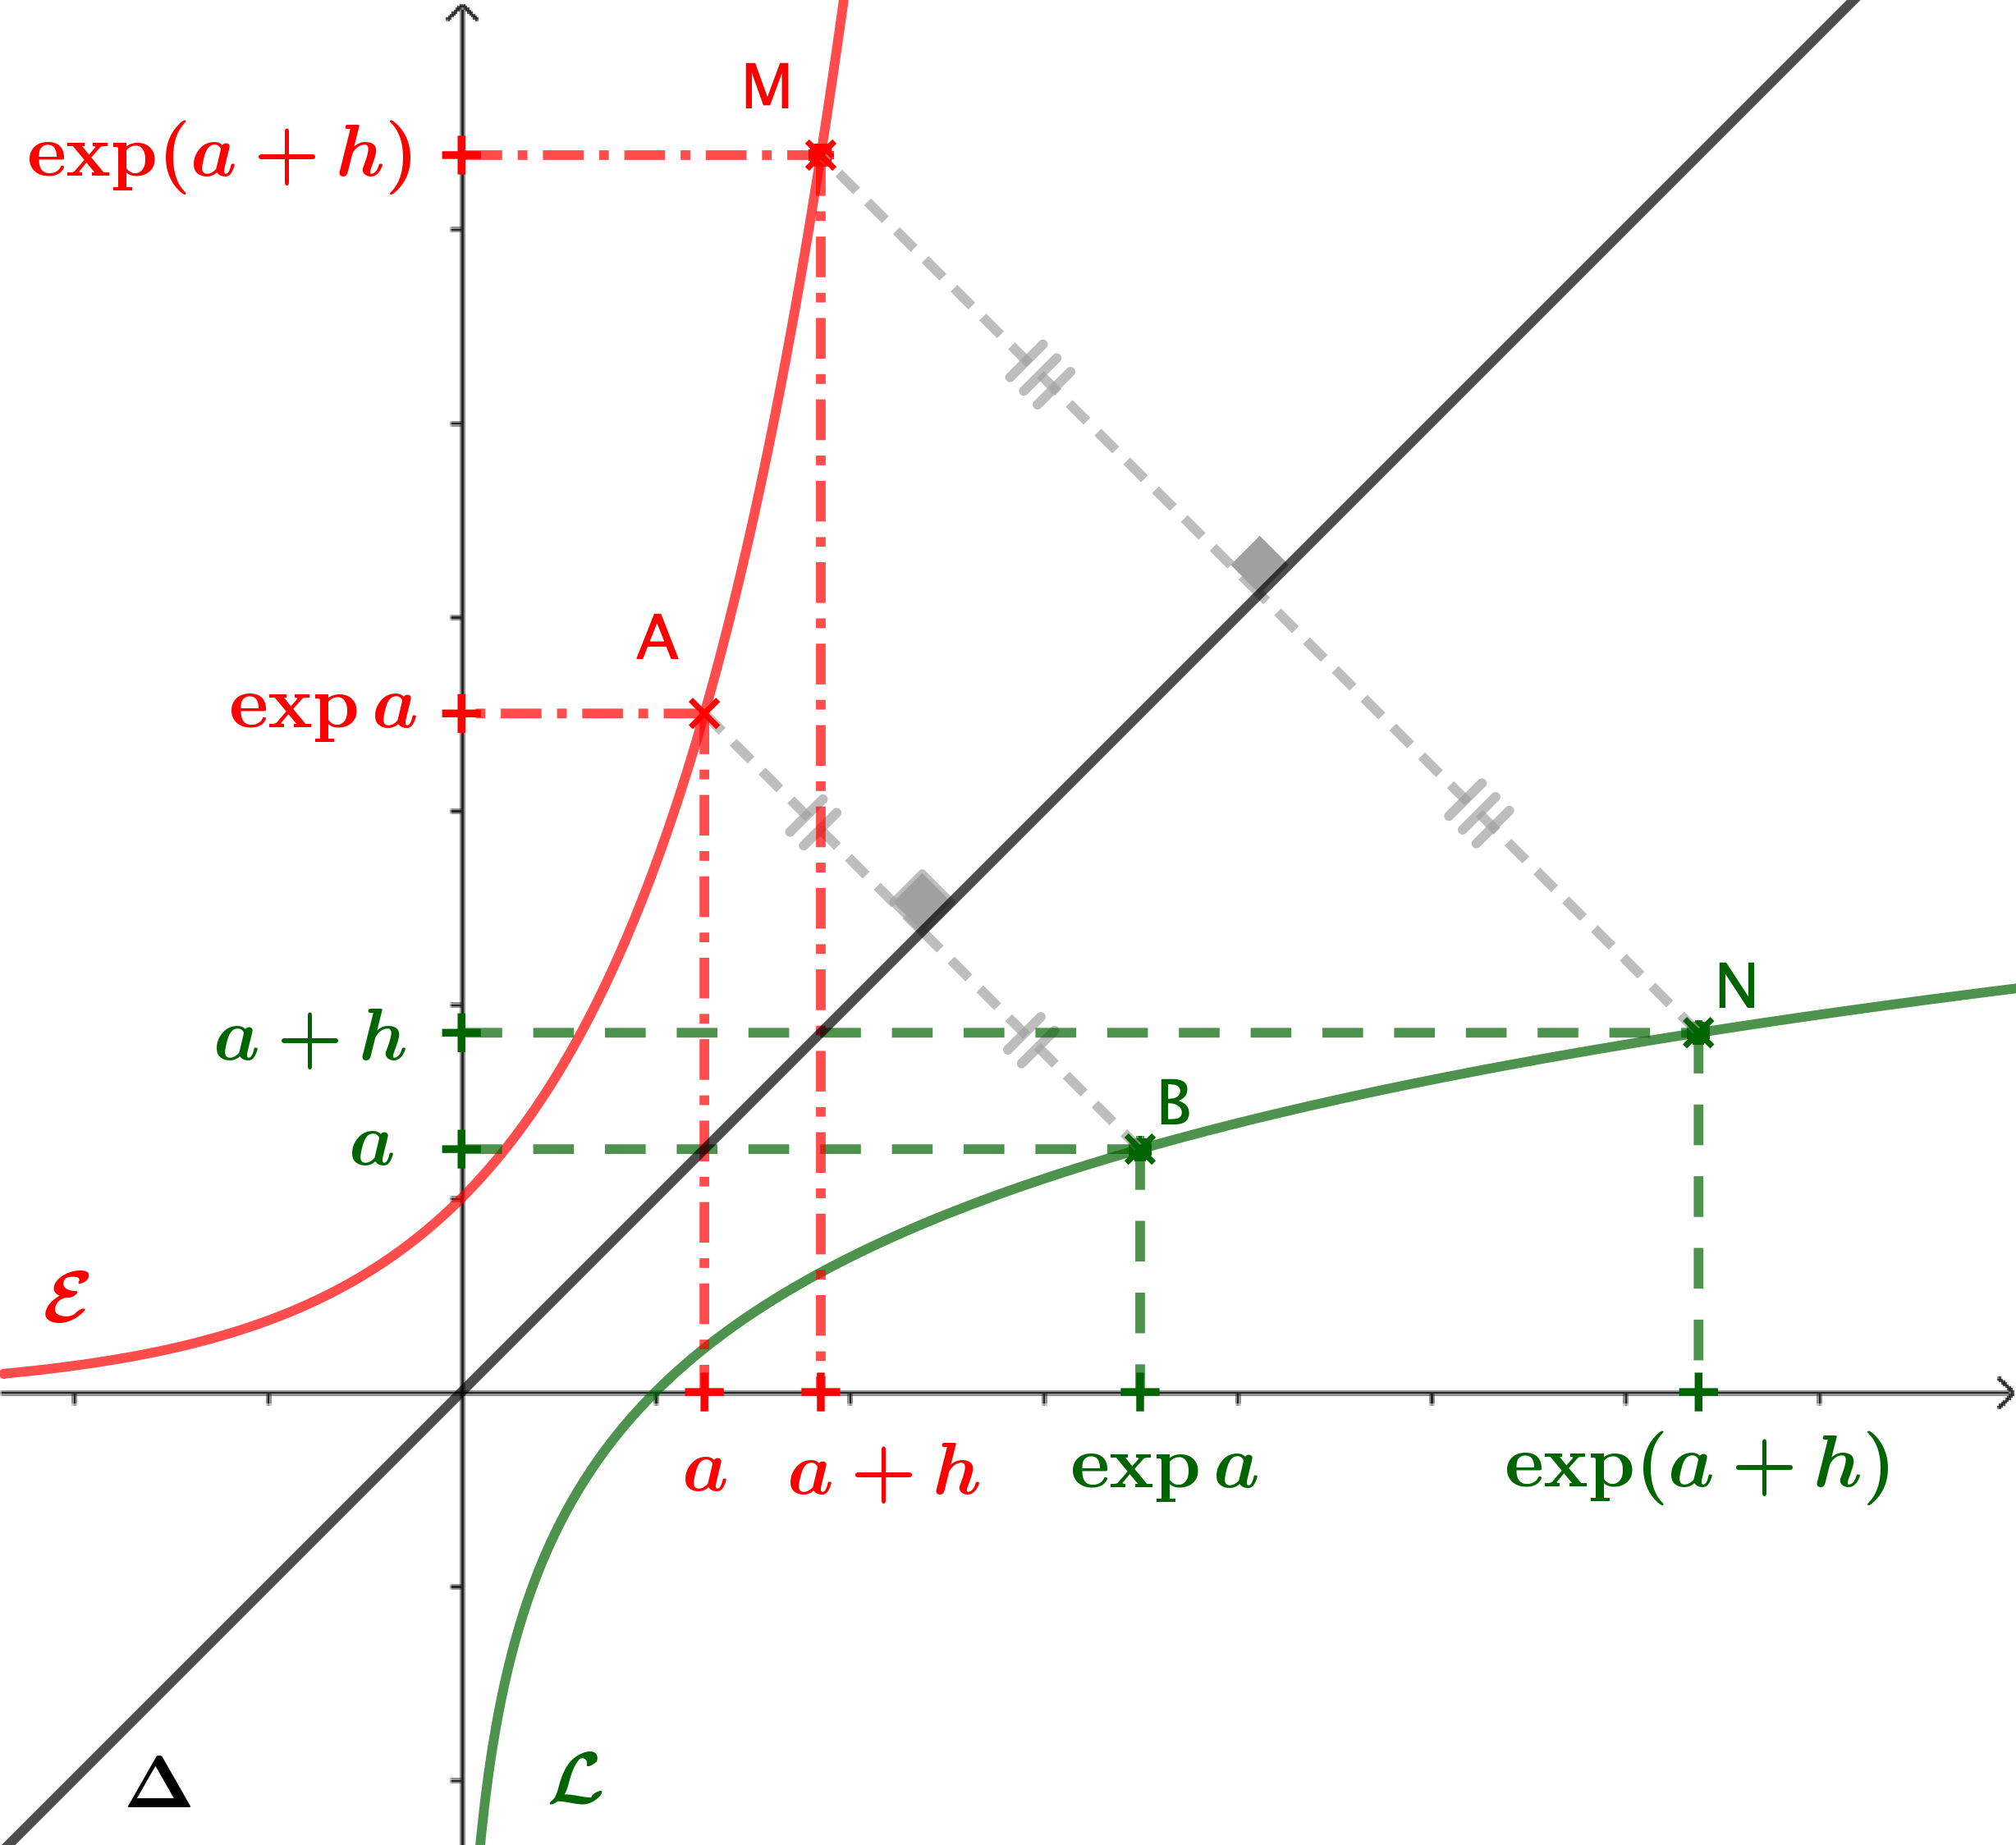
\includegraphics[scale=.85]{content/exp/eq-diff.png}
    \end{center}

    Le taux d'accroissement $T(h) = \frac{\exp(a+h) - \exp a}{h}$ est la pente $m(AM)$ de la droite $(AM)$, or $m(AM) = \frac{1}{m(BN)}$ par raison de symétrie.
    %
    En raisonnant sur $\setproba{L}$, si $h$ tend vers $0$, nous avons $x(N)$ qui tend vers $x(B)$ par continuité de $\exp$, voir le \reffact{exp-cont}.
    Comme $\ln$ est dérivable en $x(B)$, nous avons
    $\limit{m(BN)}{h}{0} = \der{\ln}{x}{1}(x(B)) = \frac{1}{\exp a}$,
    puis
    $\limit{T(h)}{h}{0} = \exp a$
    comme souhaité.
\end{proof}
